\subsection{RoleManager}\label{sec:mit-roleManager}
Orchestrating the roles is the main responsibility of the \lstinline|RoleManager| (\vref{fig:mit-roles})

\begin{figure}
\centering
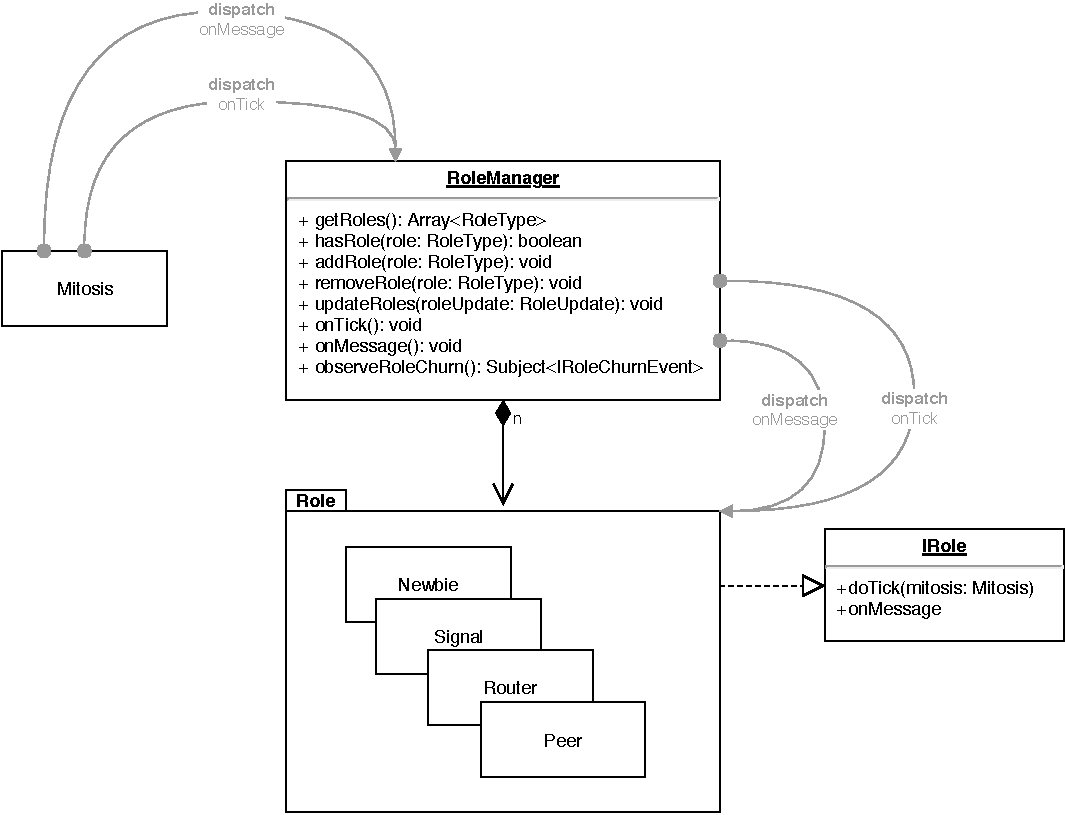
\includegraphics[width=0.75\textwidth]{graphics/implementation/mitosis-architecture-roles.pdf}
\caption{RoleManager and Roles}
\label{fig:mit-roles}
\end{figure}

The RoleManager receives \lstinline|onTick| and \lstinline|onMessage| calls from \lstinline|Mitosis-Core| and delegates them to all roles. Each role can act accordingly and execute tasks as described in \todo{reference design chapter}. 

Roles have responsibilities and desires. The rolemanager is contacting the roles whenever it receives a tick or a message so a role can execute its intention according to its belief and desire.